\section{Method 30\%}
Our method is composed of two consecutive operations: detection and classification. For the first one we adopted YOLO, an one-stage detector based on CNNs able to predict bounding boxes from input images directly without a region proposal step, achieving time efficiency and high inference speed. Therefore, it can be used not only for image detection but also for real-time devices. For the latter we built a multi-class classifier which receives as input the object detected. The reason why we don't adopt YOLO for the whole process is linked to the fact that there is a large number of classes to which a traffic sign could belong. Build a network capable of execute both detection and recognition requires a very long training time and one or more accurate and deep datasets.\\ 
One significant aspect that contributed to the choice of YOLO is the fact that it is a young framework constantly updated and supported by its team. In fact, the version used for this project is YOLOv3 \cite{yolov3}, released in 2018. The latest version, YOLOv4 \cite{yolov4}, was published on April 2020 but the lack of papers and projects to compare our results with lead us to choose the v3. 

\subsection{YOLO network setup}
To execute detection we setup the YOLO network in order to make it works with traffic signs and performs feature extraction. Its structure is composed of 53 convolutional layers with some shortcut connections which create a much more powerful network than the one used for the previous version YOLOv2. Despite being a bigger and deeper network, it is still more efficient than ResNet-101 or ResNet-152. Following this configuration the network has been pre-trained with a custom dataset. This process took many hours and produced a set of weights which, afterwards, have been given as input to build the correct network. For this purpose we use OperCV's \texttt{readNet} method. We also refer readers to explore YOLOv3 wiki\footnote{\url{https://github.com/AlexeyAB/darknet/wiki}} for its configuration and its weights. We also tried to setup the detector with a faster and smaller architecture called tiny-YOLO \cite{tinyYolo} whose performances are described in the next section.
\begin{figure}[h]
	\centering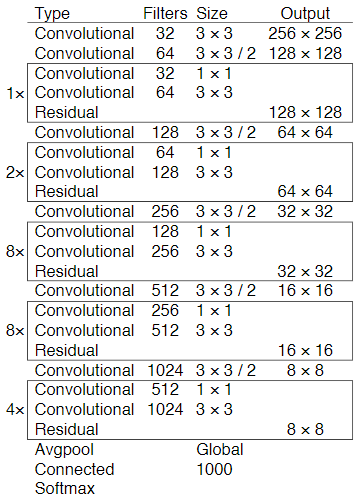
\includegraphics[scale=0.7]{Res/Immagini/darknet53.PNG}	
	\caption{Yolov3 structure (Darknet-53)}
\end{figure}

\subsection{YOLO algorithm}
%\begin{figure}[h]
%	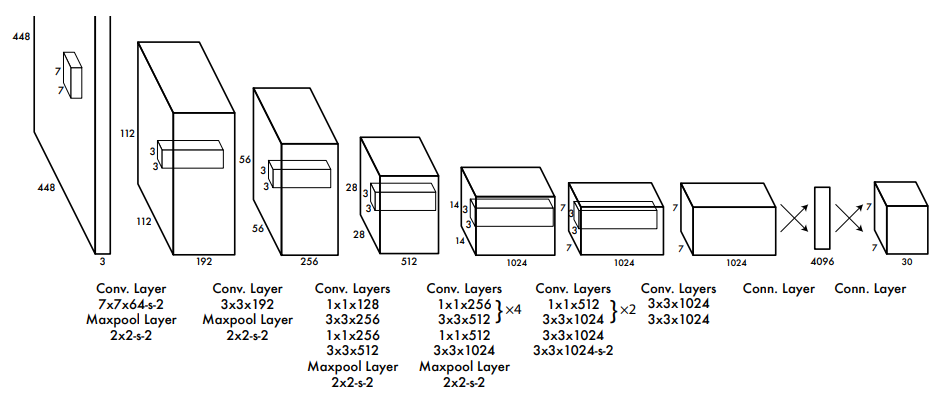
\includegraphics[width=\linewidth]{Res/Immagini/yoloArch.PNG}	
%	\caption{YOLO architecture}
%\end{figure}
The algorithm divides the input image into a $S$x$S$ grid. Each cell predicts the location of B bounding boxes, a confidence score and a probability of object class conditioned on the existence of an object in the bounding box. 
\begin{figure}[h]
	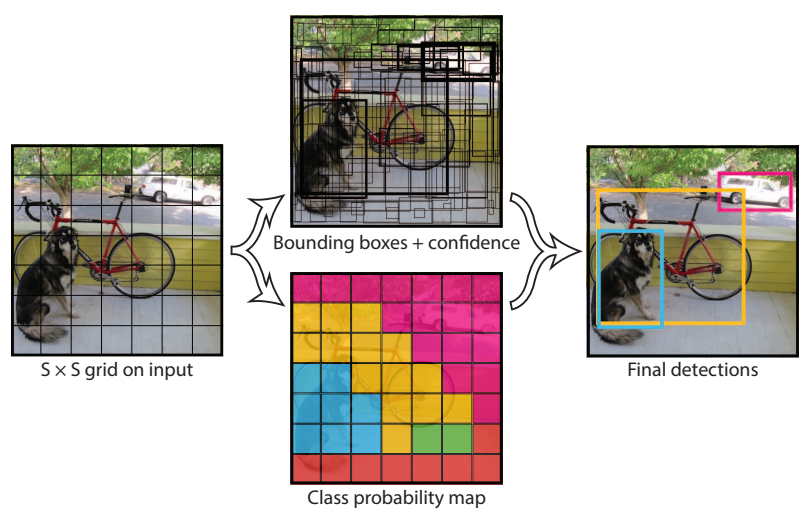
\includegraphics[width=\linewidth]{Res/Immagini/yoloAlg.PNG}	
	\caption{Workflow of YOLO}
\end{figure}
At training time one predictor is responsible for predicting an object based on which prediction has the highest current IOU (Intersection Over Union) with the ground truth. This leads to specialization between the bounding box predictors. Each predictor gets better at predicting certain sizes, aspect ratios, or classes of object, improving overall recall.\\
After that, each traffic sing is extracted, cropping the original image through coordinates of its predicted bounding box, and passed ad input to the classifier. Image detection and real-time detection can be performed using respectively \texttt{image\_analysis} method and \texttt{video\_analysis} method.

\subsection{Classification}
Our classification process is based on Keras\footnote{\url{https://keras.io/}}. In particular, we rely on Keras sequential model. It allows us to create models layer by layer in a step by step fashion. Keras provides also another type of model: the functional model. It is flexible as each layer can be connected in a pairwise fashion and can create complex networks. Since this was our first approach, we built and trained different convolutional neural networks through the sequential procedure which was easier to implement; nevertheless the results we gained are satisfying.\\
Our reference model called CNN3 is composed of 26 layers. The structure of the first 6 ones is repeated 3 times: two consecutive 2D convolutional layers with ReLu activation function each and $3$x$3$ kernel size, a layer for 2D max pooling operation and finally a layer for the dropout. The inputs are then flattened and pass through some dense layers. The other models, CNN1 and CNN2, are a simplified version of CNN3. We also implemented the LeNet architecture to test our classifier with a known convolutional neural network and to compare our experiments.

%------------------------------------------------------------------------